\chapter{Un poco de lógica}

\lettrine[ante=\raisebox{-1.5ex}{\large ---},lines=2]{A}{hora que ya}
sabemos prender todos los pixeles de un arreglo rectangular, debemos
ser capaces de elegir cuáles apagar y cuáles dejar encendidos
---Antonia comenzó sin rodeos el capítulo.

\begin{figure}[ht]
  \centering
  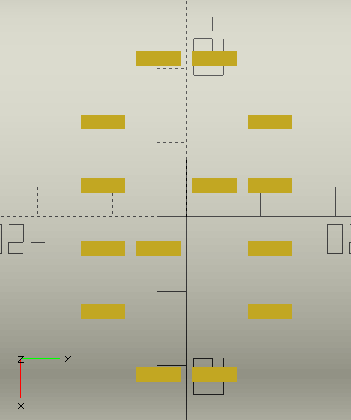
\includegraphics[height=.3\textwidth]{imagenes/cero}
  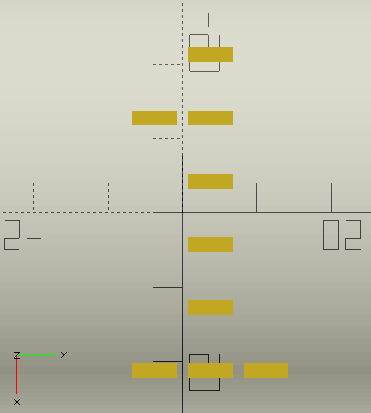
\includegraphics[height=.3\textwidth]{imagenes/uno}
  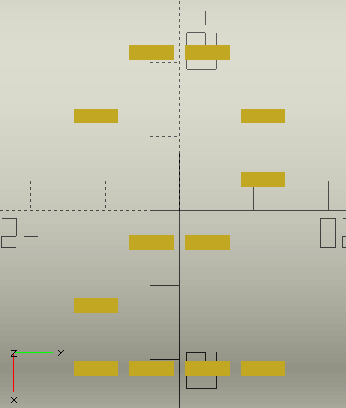
\includegraphics[height=.3\textwidth]{imagenes/dos}  
  \caption{Algunos digitos solares.}
  \label{fig:digitos-solares}
\end{figure}




\section{Condiciones}

\guillemotright Para crear objetos de acuerdo a la veracidad o no de
una cierta condición se emplea la sentencia \lstinline!if! ---dijo
Antonia mientras escribía el ejemplo de la figura \ref{fig:if-1}.

\begin{figure}[ht]
\begin{minipage}[]{.5\textwidth}%\vspace{0pt}
    \begin{lstlisting}
$fn=50;

if (1+1==2) {
  cube([5,5,5], center=true);
  translate([0,0,5])
    sphere(r=2.5);
}
\end{lstlisting}%$
\end{minipage}
\begin{minipage}[]{.49\textwidth}%\vspace{0pt}

  \centering
  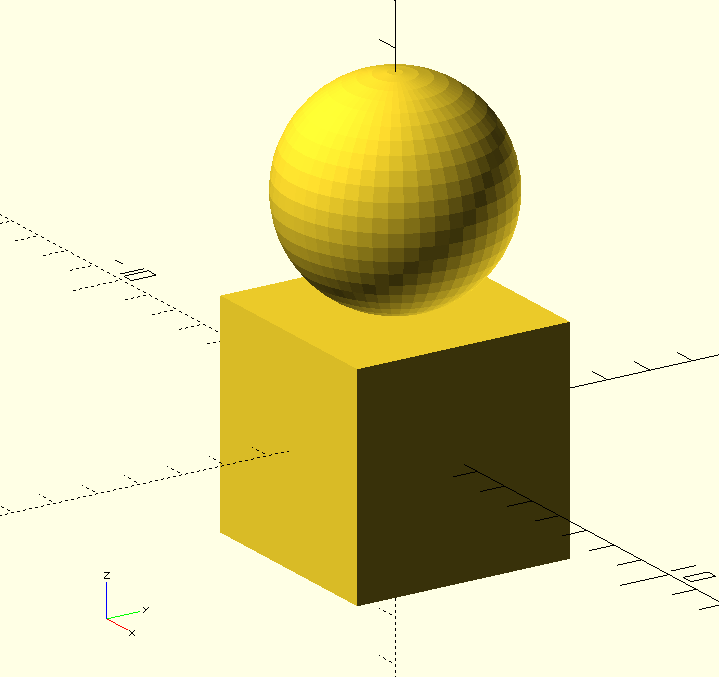
\includegraphics[width=.7\textwidth]{imagenes/if-1}
  \end{minipage}
  \caption{Primer ejemplo del uso de \lstinline!if!.}
  \label{fig:if-1}
\end{figure}


\guillemotright \lstinline!if! debe ir seguido por una condición a
verificar escrita entre paréntesis. En el caso del ejemplo, se trata
de la indiscutible aseveración de que $1+1=2$.\footnote{Alfred North
  Whitehead y Bertrand Russell ofrecen una demostración de tan
  particular aserto en la página 86 del segundo volumen de sus
  \emph{Principia Mathematica}. El primer volumen consta de unas 700
  páginas. (Nota del Editor)}

---¿Por qué en la línea 3 usaste dos veces el signo `\texttt{=}'?
---pre\-gun\-tó Cecilia.


\begin{figure}[ht]
\begin{minipage}[]{.5\textwidth}%\vspace{0pt}
  \begin{lstlisting}
$fn=50;
    
if (2+2==5) {
  cube([5,5,5], center=true);
  translate([0,0,5])
    sphere(r=2.5);
}
\end{lstlisting}%$
\end{minipage}
\begin{minipage}[]{.49\textwidth}%\vspace{0pt}

  \centering
  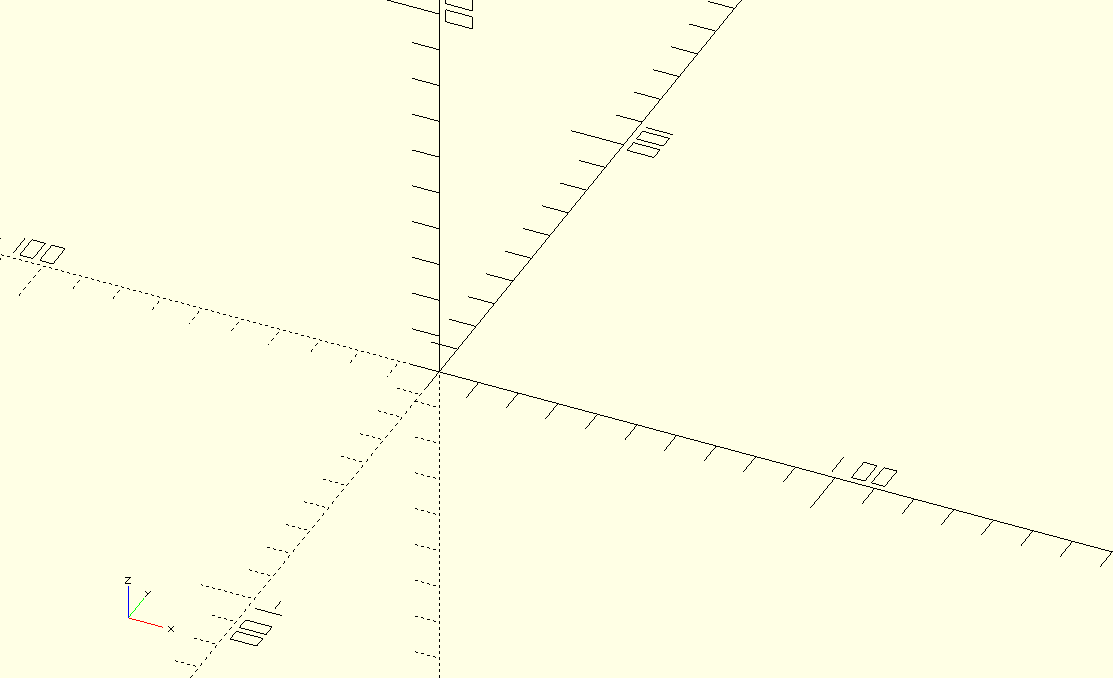
\includegraphics[width=.7\textwidth]{imagenes/vacio}
    \end{minipage}
  \caption{Resultado de un \lstinline!if! falaz.}
  \label{fig:if-vacio}
\end{figure}

---Porque un solo signo `\texttt{=}' se usa exclusivamente para las
asignaciones de variables ---justificó Antonia, y
pro\-si\-\mbox{guió---}: Si la condición es verídica, \openscad{} pasa
a concretar los objetos escritos entre llaves. Si no, los ignora
olímpicamente, como podés comprobar en la figura \ref{fig:if-vacio}.

\section{\texttt{else}}

\guillemotright También puede resultar útil, a veces, indicar diversos
objetos a realizar tanto si una condición es cierta como si es falsa:

  \begin{figure}[ht]
\begin{minipage}[]{.5\textwidth}%\vspace{0pt}
\begin{lstlisting}
$fn=200;

if (1<0) {
  cube([5,5,5]);
} else {
  sphere(r=2.5);
}
\end{lstlisting}%$

\end{minipage}
\begin{minipage}[]{.49\textwidth}%\vspace{0pt}

  \centering
  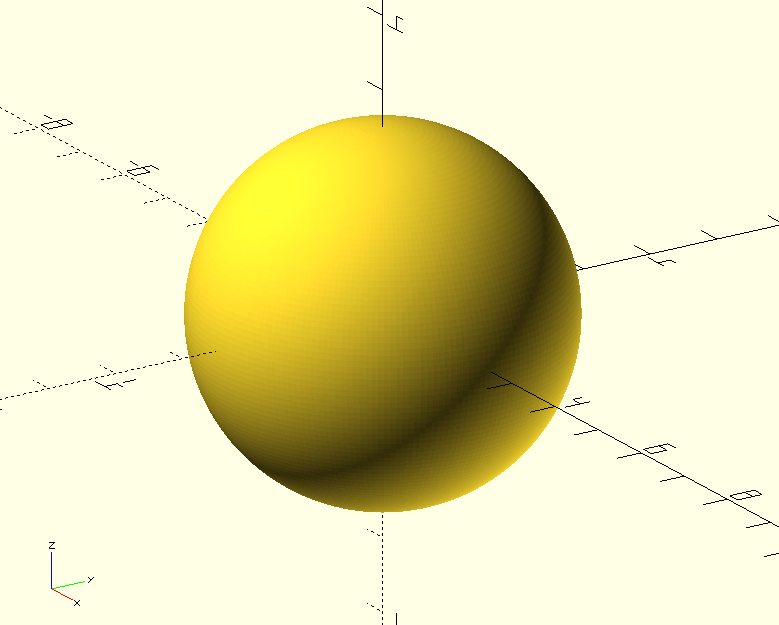
\includegraphics[width=.7\textwidth]{imagenes/if-2}
      \end{minipage}
      \caption{Uso de la construcción \lstinline!if/else!.}
      \label{fig:if-2}
\end{figure}


\guillemotright En el ejemplo de la figura \ref{fig:if-2}, si 1 fuera
menor a 0 hubiéramos visto aparecer un cubo; pero como la matemática
nos promete que no es así, fue creada una esfera ---aclaró
Antonia---. Es posible, incluso, escoger entre más de dos
posibilidades con el empleo del giro lingüístico \lstinline!else if!.

  \begin{figure}[ht]
\begin{minipage}[]{.5\textwidth}%\vspace{0pt}
\begin{lstlisting}
$fn=200;

if (1+1<2) {
  cube([5,5,5]);
} else if (1+1>2) {
  sphere(r=2.5);
} else if (1+1==2) {
  cylinder(h=5,r=2.5);
}
\end{lstlisting}%$

\end{minipage}
\begin{minipage}[]{.49\textwidth}%\vspace{0pt}

  \centering
  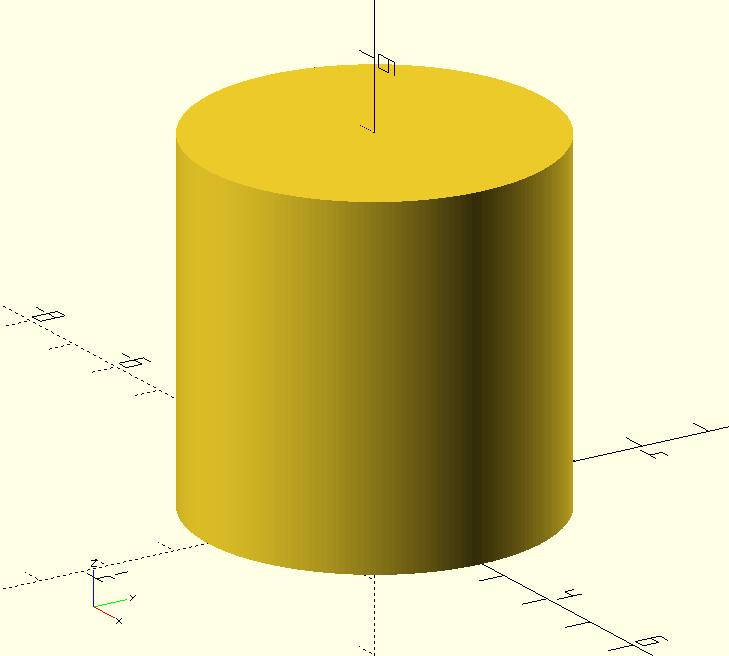
\includegraphics[width=.7\textwidth]{imagenes/if-3}
  \end{minipage}
  \caption{Antonia propone un ejemplo de la construcción
    \lstinline!else if!.}
  \label{fig:if-3}
\end{figure}

Cecilia no necesitó en este caso de la explicación de Antonia al
enfrentarse a la figura \ref{fig:if-3}: pudo ver que si $1+1$ hubiera
sido menor que 2, habría sido creado un cubo. Como no fue así,
\openscad{} pasó a comprobar si $1+1$ era mayor que 2. En caso
afirmativo, hubieran visto una esfera; pero como no era el caso, se
verificó luego si $1+1$ era igual a 2. Ante la indiscutible veracidad
del hecho, \openscad{} no tuvo más remedio que crear un cilindro.

---¿Qué pasa si varias condiciones son ciertas? ---preguntó Cecilia.

---Se crean los objetos sujetos a la primera que lo sea; los demás se
ignoran ---res\-pon\-dió Antonia. Sin embargo, tras un momento, añadió:
---Bah, así debería ser, supongo; vamos a comprobarlo por las dudas.

  \begin{figure}[ht]
\begin{minipage}[]{.5\textwidth}%\vspace{0pt}
\begin{lstlisting}
$fn=200;

if (1+1==2) {
  cube([5,5,5]);
} else if (2+2==4) {
  sphere(r=5);
} else if (1*1==1) {
  cylinder(h=5,r=5);
}
\end{lstlisting}%$
\end{minipage}
\begin{minipage}[]{.49\textwidth}%\vspace{0pt}

  \centering
  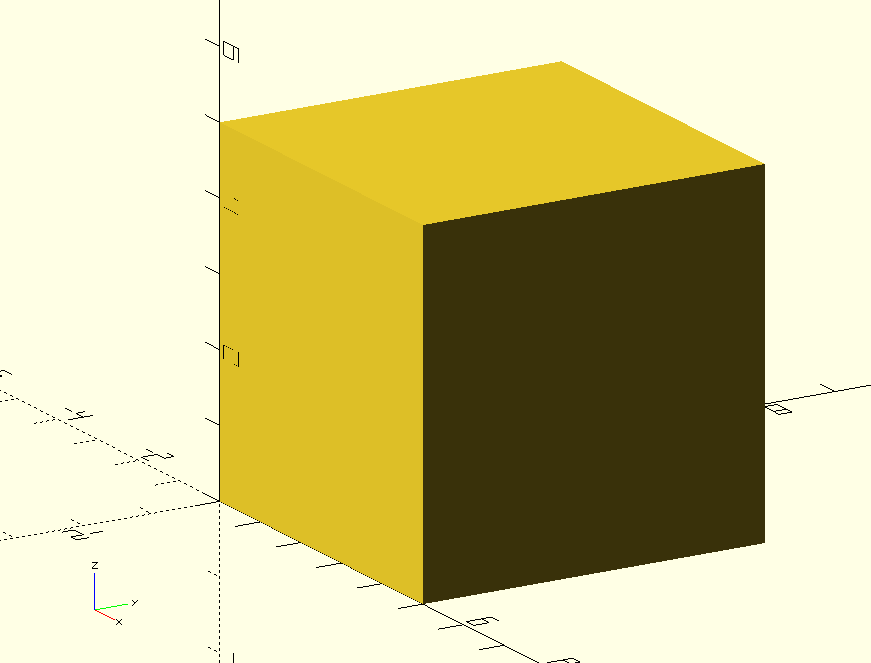
\includegraphics[width=.8\textwidth]{imagenes/if-4}
\end{minipage}
\caption{Antonia comprueba una conjetura acerca del funcionamiento de
  varios \lstinline!else if!.}
\label{fig:if-4}
\end{figure}


\guillemotright Y así era, nomás ---concluyó con una sonrisa ante la
figura \ref{fig:if-4}.

\section{Conectores lógicos}

---Hay más comparadores, por supuesto, como `\lstinline!>=!'  (mayor o
igual), `\lstinline{<=}' (menor o igual) y `\lstinline{!=}' (distinto)
---prosiguió Antonia---. Por otra parte, te van a resultar
extremadamente útiles los conectores lógicos 'Y' (\lstinline!&&!) y
'O' (\lstinline!||!). El primero obliga a verificar que \emph{todas}
las condiciones entre paréntesis sean ciertas: si una sola es falsa,
los objetos se omiten:

  \begin{figure}[ht]
\begin{minipage}[]{.6\textwidth}%\vspace{0pt}
\begin{lstlisting}
if (1+1==2 && 2+2==4 && 1<0) {
  cube([5,5,5]);
}   
\end{lstlisting}
\end{minipage}
\begin{minipage}[]{.39\textwidth}%\vspace{0pt}
%\begin{figure}[ht]
  \centering
  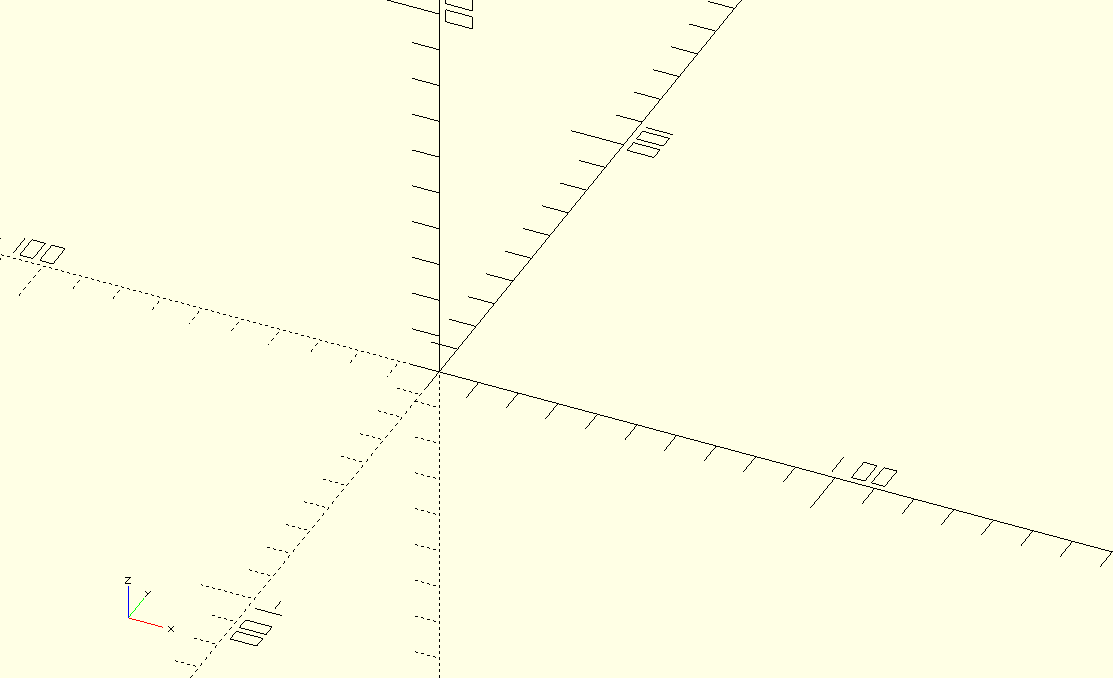
\includegraphics[width=\textwidth]{imagenes/vacio}
  \end{minipage}
  \caption{El conector lógico \texttt{\&\&} sólo da por cierto un
    conjunto de condiciones si todas lo son.}
  \label{fig:if-y}
\end{figure}

\guillemotright El cubo hubiera aparecido en la figura \ref{fig:if-y}
si $1+1=2$ \emph{y} $2+2=4$ \emph{y} $1<0$; pero como claramente la
última condición es falsa, no apareció nada ---comentó Antonia---. Por
su parte, el conector \lstinline!||!  verifica que al menos una de las
condiciones sea cierta; en ese caso, realiza los objetos entre llaves:

  \begin{figure}[ht]
\begin{minipage}[]{.6\textwidth}%\vspace{0pt}
\begin{lstlisting}
if (1+1==3 || 2+2==5 || 1>0) {
  cube([5,5,5]);
}      
\end{lstlisting}
\end{minipage}
\begin{minipage}[]{.39\textwidth}%\vspace{0pt}
%\begin{figure}[ht]
  \centering
  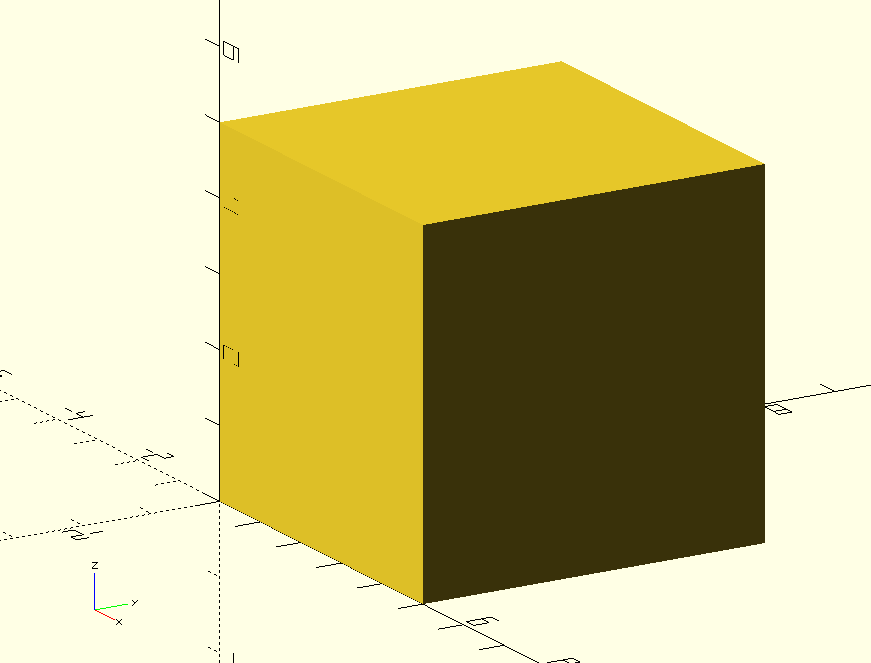
\includegraphics[width=\textwidth]{imagenes/if-4}
\end{minipage}
\caption{El conector lógico \texttt{||} da por bueno un conjunto de
    condiciones con tal que al menos una sea veraz.}
  \label{fig:if-o}
\end{figure}

\guillemotright $1+1$ no es igual a 3, ni $2+2$ será nunca 5; pero
como 1 es mayor que 0, ahí tenemos nuestro cubo ---redondeó Antonia
señalando la figura \ref{fig:if-o}---.  Este capítulo fue cortito, así
que aprovecho para comentarte que si el objeto a crear es uno solo,
podés omitir las llaves, tal como se aprecia en la figura
\ref{fig:if-sin-llaves}.


\begin{figure}[ht]
\begin{minipage}[]{.5\textwidth}%\vspace{0pt}   
\begin{lstlisting}
if (1+1==2)
  cube([5,5,5]);
\end{lstlisting}
\end{minipage}
\begin{minipage}[]{.49\textwidth}%\vspace{0pt}   
  \centering
  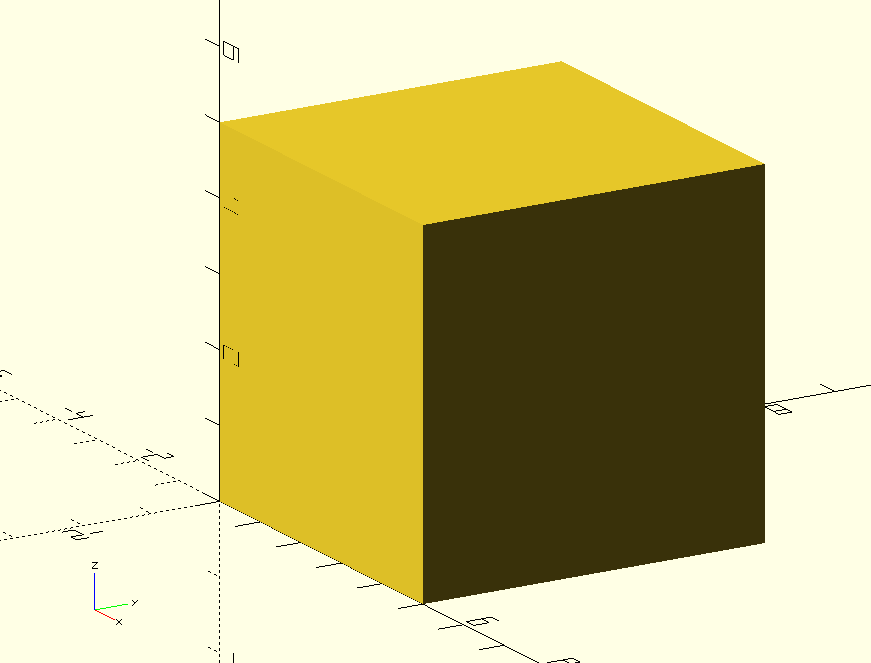
\includegraphics[width=.75\textwidth]{imagenes/if-4}
\end{minipage}
\caption{Si el \lstinline!if! rige la creación de un solo objeto,
  las llaves pueden omitirse.}
\label{fig:if-sin-llaves}
\end{figure}


Cecilia ya casi no escuchaba a Antonia, porque su mente empezó a soñar
con aprovechar lo visto en el presente capítulo para prender o apagar
los pixeles de cada dígito solar.

%%% Local Variables:
%%% mode: latex
%%% TeX-master: "../libro"
%%% End:
